We want to obtain the $\assym_{M,e,\Pr}(x_i)$. We also have the causal digraph $G$, which is a forest. We can classify the nodes into ancestors, descendants and unrelated to $x_i$. Now we want to calculate this formula : $$\assym_{M,e,\Pr}(x_i) = \heuristicASVFormula$$

For that, first we will need to calculate all the equivalence classes, one topological order of $G$ that is included in each of them and their respective sizes. We divided this algorithm into two parts, in the first one we obtain the equivalence classes for the unrelated trees and in the second one we merge this classes with the ancestors and ascendants. Here we have our forest example:

\newcommand{\drawUnrelatedTree}[4]{
    \node[unrelated] (#1) at (#2, #3) {#4};
     \pgfmathsetmacro{\x}{#2-2}
     \pgfmathsetmacro{\y}{#3-0.3} 
    \draw[red, wiggly] (#2, \y)
        -- ++(-1,-1.6) 
        -- ++(2,0) 
        -- cycle;
    \node[text=red] at (\x, \y) {#4 subtree};
}

\begin{figure}[H]
    \centering
    \begin{tikzpicture}[scale=.95, transform shape, 
    unrelated/.style={circle, draw=red},
    ancestor/.style={circle, draw=blue},
    wiggly/.style={decorate, decoration={snake, amplitude=.2mm, segment length=2mm}}  % Define wiggly line style
    ]
        \node[text=blue] at (-5, 0) {Ancestors};
        \node[text=teal] at (-5, -0.5) {Descendants};
        \node[text=red] at (-5, -1) {Unrelated};        
        
        % ---- NODOS ----

        \node[ancestor] (a1) at (0, 0) {$a_1$};
        \node[unrelated] (u1) at (-1, -2) {$u_1$};
        \node[ancestor] (a2) at (1, -2) {$a_2$};

        \drawUnrelatedTree{u2}{-1}{-4}{$u_2$}
        \node[ancestor] (a3) at (1, -4) {$a_3$};
        \node[unrelated] (u3) at (3, -4) {$u_3$};

        \drawUnrelatedTree{u4}{0}{-7}{$u_4$}
        \node[ancestor] (a4) at (3, -6) {$a_4$};

        \node[nodo] (xi) at (3, -8) {$x_i$};

        \drawUnrelatedTree{r1}{6}{0}{$u_5$} 
        \drawUnrelatedTree{r2}{10}{0}{$u_6$} 
        
        \node[draw=none, fill=none] (hi) at (3, -10) {};


         \path [->] (a1) edge[arista]  (u1);
         \path [->] (a1) edge[arista]  (a2);

         \path [->] (a2) edge[arista]  (u2);
         \path [->] (a2) edge[arista]  (a3);
         \path [->] (a2) edge[arista]  (u3);

         \path [->] (a3) edge[arista]  (c1);
         \path [->] (a3) edge[arista]  (a4);

         \path [->] (a4) edge[arista]  (xi);      
         \path [->, teal] (xi) edge[arista,  decorate, decoration={snake, amplitude=.4mm, segment length=4mm, post length=1mm}] node[right] {descendants of $x_i$} (hi);
    \end{tikzpicture}
    \caption{Example of a possible causal DAG to calculate the ASV from}
    \label{fig:ASV_forest_example}
\end{figure}



\subsection{Naive formula}

There is also a naive way to calculate this. First, we calculate all the toposorts of the forest using the algorithm proposed in \cite{KNUTH1974153}. After that, we can iterate over the toposorts and assign them to an equivalence class, depending on which unrelated nodes are before $x_i$. After that we will have our classes, a representative for each of them and their classes. The problem here is that we need to calculate explicitly each toposort of $G$, which can be $O(n!)$. 

%TODO : Find a better upper bound, one more tight

\subsection{Equivalence classes for unrelated trees}


First, we need to find the roots of these unrelated trees, we will call this set $UR$. A node $x$ will be a root of an unrelated tree if it's a root and an unrelated node, or if it's only parent is an ancestor of $x_i$. We will represent an equivalence class using a set of which unrelated nodes it has before and after $x_i$, this would be the representation of an $\eqCl = \{ n_t \mid \ n \in V(G) \land t \in  \{ left, right\} \}$. $L(\eqCl)$ and $R(\eqCl)$ will return the number of nodes to the left and to the right in the equivalence class. This algorithm will return a set of tuples with the format $(\eqCl, leftTopos, rightTopos)$. $leftTopos$ being the number of topological orders that we can make with the unrelated nodes before $x_i$ and $rightTopos$ the same but with the ones after.The notation here used is: \\
$n_i$ = $i-th$ child of node $n$, $|n|$ = the number of children of node $n$.
Then we will run this algorithm for each $node \in UR$, here is the algorithm: 

\label{formula:unrelated_equiv_classes}
%  \[
%     \unrEqCl(n) = 
%     \begin{cases} 
%     \set{(\set{n_l}, 1, 1), (\set{n_r},1,1)} & \text{if $n$ is a leaf} \\
%     (\bigcup_{\forall mix \in \unrEqCl(n_1) \times \dots \times \unrEqCl(n_{|n|})} LeftUnion(mix,n)) \cup RightUnion(right,n) & \text{oc.}
%     \end{cases}
% \]


\[
    \unrEqCl(n) = 
    \begin{cases} 
    \set{(\set{n_l}, 1, 1), (\set{n_r},1,1)} & \text{if $n$ is a leaf} \\[1ex]
    \begin{aligned}
    &\left( \bigcup_{\forall mix \in \unrEqCl(n_1) \times \dots \times \unrEqCl(n_{|n|})} \hspace{-6em} LeftUnion(mix,n)\right) \\
    &\cup RightUnion(right,n)
    \end{aligned} & \text{otherwise}
    \end{cases}
\]


%TODO: Dejar más lindo esto, esta feo así

\begin{align*}
&leftUnion(n, ((eqCl_1, lTopo_1, rTopo_1), ...., (eqCl_{|n|}, lTopo_{|n|}, rTopo_{|n|}))) = \\ 
&\left(\bigcup_{j=1}^{|n|} eqCl_j \cup \set{n_l}, \binom{\sum_{i=1}^{|n|} L(eqCl_i)}{L(eqCl_1), \ldots, L(eqCl_{|n|})} \prod_{i=1}^{|n|} lTopo_i, 
\binom{\sum_{i=1}^{|n|} R(eqCl_i)}{R(eqCl_1), \ldots, R(eqCl_{|n|})} \prod_{i=1}^{|n|} rTopo_i \right)
\end{align*}

Here $leftUnion$ represents the union of all the equivalence classes, positioning the node $n$ to the left of $x_i$. We can see the that for calculating the left and right topological orders we use the same formula as in \ref{Number Of Toposorts}. It's the same logic because there are no dependencies between the nodes of the unrelated trees and it's subtrees, so we can mix the toposorts as we like. \\
We also have $rightUnion$, which is the same as $leftUnion$, but in the first tuple it adds $n_r$ instead. It needs to use $right$ because if the node $n$ appears after $x$ \\
$right$ being the product that fulfills that, all of its nodes appear after $x_i$: \\ $right \in \unrEqCl(n_1) \times \dots \times \unrEqCl(n_{|n|}),  \forall (eqCl, \_ , \_) \in right, L(eqCl)=0$ \\

\label{slight_improvement}
There is also a slight improvement implemented, in which we unite some of the unrelated equivalence classes. Let's imagine that we have the results for $\unrEqCl(ur_1)$ and $\unrEqCl(ur_2)$. If $ur_1$ and $ur_2$ have both the same parent or are both roots, then we will unite them. That's because when we are doing the $leftOrders$ calculation, it does not matter if a node comes from either subtree, since they both depend on the same $ancestor$. This optimization will make it so that in $leftOrders$ we have less permutation to calculate. What we do is similar as if in the \ref{fig:ASV_forest_example} we added a virtual node $v$, which is the parent of $u_5$ and $u_6$, and then ran $\unrEqCl$ from it, using only the $leftUnion$ (cause this node does not exist). 

\subsection{Merging of unrelated trees classes with ancestors and descendants}

Now we need to combine the previous classes obtained and merge them with the ancestors and descendants of $x_i$. \\

Foremost, why can't we use the previous formula and just merge them as we were doing before? Let's imagine that we didn't and we just use the $leftUnion$ with the ancestors. The tuple that represents them will be $(\set{ a_l | a \in A}, 1, 1)$, $A$ = $ancestors$. This is because they only have one possible order, and all of them must appear before $x_i$. Now if we used, $leftUnion$ we would be doing this calculation $\binom{|A| + |U|}{|A|}$, that means that we could insert the elements of $A$ between any element of $U$ in the topological order, but that is incorrect! Because in this scenario, there are dependencies between the nodes. In the example \ref{fig:ASV_forest_example} we cannot put $u_1$ before $a_2$ or any of the nodes in the $u_2$ subtree before $a_2$. That means that we need another function to calculate the possible orderings of the nodes that appear before $x_i$ and the ancestors. We are going to call this function $leftOrders$. \\
Now the question is, what do we do with the descendants? Here we are not restricted as we were before with the ancestors, so we can use the same formula that we were using. Because there are no dependencies between the nodes in $D$ and $UR$.\\
Taking that into account, we can finally define the last step. $u_i$ will be root node of the $i-th$ unrelated tree. This is our formula, for calculating all the equivalence classes and their sizes in a forest: 

\label{formula:equiv_classes_sizes}
\[
    \eqClassSizes(G) = 
    \bigcup_{\forall mix \in \unrEqCl(u_1) \times \dots \times \unrEqCl(u_{|UR|})} \left( eqCl(A,D, mix) , \#eqCl(A,D,mix) \right) 
\]

%TODO: Dejar más lindo esto, esta feo así

\begin{align*}
eqClass(A, D, ((eqCl_1, \_ , \_ ), ...., (eqCl_{|UR|}, \_ , \_))) &=  \set{a_l \mid a \in A} \cup \set{d_r \mid d \in D} \cup (\bigcup_{j=1}^{|UR|} eqCl_j) \\ 
\#eqClass(A, D, mix) &= leftSize(A,mix) * rightSize(D, mix)  \\ 
\#leftSize(A, ((eqCl_1, l_1, \_), ...., (eqCl_{|UR|}, l_{|UR|}, \_))) &= leftOrders(A, [ l_1, \dots, l_{|UR}]) * \prod_{i=1}^{|UR|} l_i  \\
\#rightSize(D, ((eqCl_1, \_, r_1), ...., (eqCl_{|UR|}, \_, r_{|UR|} ))) & = \\ & \hspace{-1.5cm} \binom{|D| + \sum_{i=1}^{|n|} R(eqCl_i)}{R(eqCl_1), \ldots, R(eqCl_{|n|}), |D|} * \prod_{i=1}^{|UR|} r_i * \numTopo(x_i)
\end{align*}

Let's explain the possible combinations. In $eqClass$ we put nodes in $A$ before $x_i$ and the nodes in $D$ after, since it's the only possible combination. In, $\#eqClass$ we obtain the size by multiply all the left topological orders with the right one, because a combination of both will still respect the equivalence class.  For, $rightSize$ we used the same formula as before and just added the topological orders of the descendants using the formula of \ref{Number Of Toposorts}. And for $leftSize$ we calculated the possible combinations using the function from here below. 

\subsubsection{Combinations of left nodes and ancestors}

These are the variables that we are going to take into account to calculate the various combinations. The $ancestors$, the value of $L(eqCl)$ for each $eqCl$ of its corresponding unrelated tree and the root of each unrelated tree. What we want to do is define the number of toposorts that we can make, combining the nodes to the left of each unrelated tree and the ancestors.  Let's see an example with \ref{fig:ASV_forest_example}, what orders can we generate with nodes from $A$ positioned like this:

%TODO: Agregar una ilustración más copada. 
\begin{figure}[ht]
    \centering
    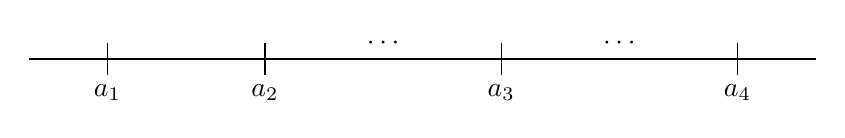
\begin{tikzpicture}
        % Draw the main line
        \draw[thick] (0,0) -- (10,0);
        
        % Draw and label the points
        \foreach \x/\label in {1/$a_1$, 3/$a_2$, 6/$a_3$, 9/$a_4$} {
            \draw (\x,0.2) -- (\x,-0.2); % Ticks
            \node[below] at (\x,-0.2) {\label}; % Labels
        };
        
        % Dots in between
        \node at (4.5,0.2) {$\cdots$};
        \node at (7.5,0.2) {$\cdots$};
    \end{tikzpicture}
    \caption{Possible ordering of the ancestors}
    \label{fig:order_of_ancestors}
\end{figure}

Now the question is, where can we place the elements of each unrelated tree. Before, $a_1$ we can only put nodes that are in the $u_5$ or $u_6$ subtree. Before $a_2$ we can put the same elements, plus $u_1$. In general, before a node $a_i$ we will be able to put all the nodes that are included in an $unrelated \ tree$ that it has root $ur$ such that $ur$ is a root or $a_j$ is the parent of $u_r$, with $j<i$. Now we want to turn this into a recursive formula so that we can use dynamic programming to solve this problem, as there are going to be multiple instances of overlapping problems. \\
For the algorithm, what we will be doing will in each step will be:
\begin{enumerate}
    \item Define where are we going to place the next ancestor. 
    \item Select how many nodes from each unrelated tree we are going to use to fill all the positions.
    \item Remove the selected nodes from our possible options to choose from. 
    \item Start the recursion again. 
\end{enumerate}
The parameters of the function will be:
\begin{itemize}
    \item $p$: position in which the last ancestor was placed
    \item $i$: index of the ancestor that we are going to place
    \item $nodesPerAncestor$: a list which has, in the $i-th$ position, the number of nodes to the left of the unrelated tree of $a_i$.
        \begin{itemize}
            \item Because of the slight improvement mentioned in \ref{slight_improvement} there will only be one tree under each $a_i$, since they are being merged into one. 
         \end{itemize}
\end{itemize}
We will also have some auxiliary functions: 
\begin{itemize}
    \item $\mathrm{possibleCombinations}(l,i,nodesPerAncestor) \ \text{or} \ pb$, which returns all the possible ways that you can sum the first $i$ elements of $nodesPerAncestor$ to obtain $l$. 
        \begin{itemize}
            \item For example, $\mathrm{possibleCombinations}(4,2,[10,2,6,7, \dots])= [[4,0], [3,1], [2,2]]$. 
        \end{itemize}
    \item $\mathrm{hasPlaced}(placedNodes, nodesPerAncestor) \ \text{or} \ hp$, returns a list $l$ which has in the $i-th$ position the element $l[i]= nodesPerAncestor[i] - placedNodes[i]$.
    \item $\mathrm{canPlace}(nodesPerAncestor, i) \ \text{or} \ cp$, returns the sum of the first $i$ elements of $nodesPerAncestor$.
\end{itemize}
Using this logic, our function will be like this: 

\label{formula:left_possible_orders}
%  \[
%     \leftPossibleOrders(p,i,npa) = 
%     \begin{cases} 
%     \sum_{comb \in pb(cp(i,npa),i, npa)} \binom{ sum(comb)}{comb_1, \ldots, comb_i} & \text{if $|A|=i$} \\
%     \sum_{s=p}^{p+cp(i,npa)} \sum_{comb \in pb(s-p-1,i, npa)} (\binom{ sum(comb)}{comb_1, \ldots, comb_i} * \leftPossibleOrders(s,i+1,hp(comb, npa))  & \text{otherwise}
%     \end{cases}
% \]

 \[
    \leftPossibleOrders(p,i,npa) = 
    \begin{cases} 
    \sum_{comb \in pb(cp(i,npa),i, npa)} \binom{ sum(comb)}{comb_1, \ldots, comb_i} & \text{if $|A|=i$} \\[2ex]
    \begin{aligned}
    &\sum_{s=p}^{p+cp(i,npa)} \sum_{comb \in pb(s-p-1,i, npa)} \Big(\binom{ sum(comb)}{comb_1, \ldots, comb_i} \\
    &  * \leftPossibleOrders(s,i+1,hp(comb, npa)\Big)
    \end{aligned}
    & \text{otherwise}
    \end{cases}
\]


%Esto en realidad es más complejo, hay algunas transformaciones que se tienen que hacer a left. ¿Las anoto o no tiene sentido? (Es lo que se hace en leftElementsOfClasses en el código)

In the otherwise case, the $s-p-1$ is the number of positions that we need to fill between the $a_i$ that we are placing and the $a_{i-1}$ that was placed before. Now with all this function defined, the call that will solve $leftOrders(A, left)$ will be $f(0,0,left)$. We implemented this function using dynamic programming, so we won't be solving the overlapping problems twice. 


\subsection{Time complexity}
%TODO: ¿Esta es la idea? ¿Cuánto más formal debería ser? ¿Cuánto mejor lo debería escribir? ¿Busco una cota un poco más fina?
Let $n$ be the number of nodes of the causal digraph $G$, $r$ the root of $G$ and $eq$ the number of equivalence classes in $G$ for feature $x_i$.

\subsubsection{Time complexity of \unrEqCl}

For calculating the complexity of \unrEqCl, defined in \ref{formula:unrelated_equiv_classes}, we are going to calculate how much each node costs and how many calls there are. $leftUnion$ and $rightUnion$ does 4 times $|n|$ operations of cost $O(1)$, 2 $\prod \ and \ \sum$. The multinomial coefficient is $O(n)$ in the worst case, so $leftUnion$ and $rightUnion$ will have a $O(n)$ time complexity. Then we need to bound the number of $mix$ that will be created in each call, but because we are generating the equivalence classes here we know it will be bounded by $\#equivalenceClasses$. We will also call this function at most $n$ times, once for each node. That leaves us with a total time complexity of $O(n^2 * \#equivalenceClasses)$.

\subsubsection{Time complexity of \#eqClass}

First, we need to calculate the time complexity of $rightSize$, which is $O(n)$. We have the multinomial coefficient, which takes $O(n)$ time, the $\prod$ which is $O(n)$ cause $|UR|<n$ and $\#topo(x_i)$ which can be implemented in $O(n)$. Then the sum of 3 operations that take $O(n)$ time is $O(n)$. 

%TODO: Revisar la cota de complejidad para \#topo(x_i), cómo mucho va a ser  $O(n^2) igual$

We also have to calculate the complexity of \leftPossibleOrders, defined in \ref{formula:left_possible_orders}, for that we need to know how much does it cost to calculate each node and how many possible states there are.

Let's start with the possible states. We have the parameters $i$, $p$ and $nodesPerAncestor$. $i$ has $|A|$ possible values, which in the worst case is $O(n)$. $p$ can take $O(n)$ possible values in the worst case, because a topological order can have at most $n$ nodes. Now we have to  calculate the number of possible states for $nodesPerAncestor$: 

For each $i$ position, we are going to have the number of nodes to the left of the unrelated trees under $a_i$. Let $size(ut_i)$ be the size of the unrelated tree $ut_i$ under node $a_i$ (if there is none, it is 0). For the $i-th$ position, we have $size(ut_i)$ possible values. But with formula \ref{formula:number_of_equiv_classes} we know that $\numEqCl(ut_i) > size(ut_i)$, that means that the possible values of $nodesPerAncestor$ are bounded by $\prod_{i=0}^{|A|} size(ut_i) < \prod_{i=0}^{|A|} numEqCl(ut_i)$. And knowing how we calculate all the equivalence classes sizes in \ref{formula:number_of_equiv_classes} we know that $\prod_{i=0}^{|A|} numEqCl(ut_i) < numEqCl(r) = \text{number of equivalence classes}$. With that, we can conclude that $\# possible \ values \ of \ npa < number \ of \ equivalence \ classes$. 

%TODO: Creo que cometí un crimen de lesa humanidad metiendo la notación O acá, pero después lo corrijo.
Then we have that the number of states is in the order of $values(i) * values(p) * values(npa) = O(n) * O(n) * \#equivalenceClasses = O(n^2 * \#equivalenceClasses)$.

Now we need to calculate how much does each node costs. The multinomial coefficient is $O(n)$, because the maximum size $comb$ can take is $n$ and multiplying is $O(1)$. So the number of sums will determine our complexity. $s$ can take at most $\sum_j^i size(ut_j)$ values in each iteration, and that's bounded by $n$. The question is how many values can $\mathrm{possibleCombinations}(l,i,nodesPerAncestor)$ can take. We know that for each result $res$ such that $res \in pb(l,i,npa), \forall 0<j<|res|, 0<res[j]<npa[j]$. So using a similar argument as the one in $nodesPerAncestor$ we can conclude that $pb(l,i,npa) < \#equivalenceClasses$. Concluding that the cost of calculating each state is $O(n^2 * \#equivalenceClasses)$.
Now we need to calculate how much does each node costs. The multinomial coefficient is $O(n)$, because the maximum size $comb$ can take is $n$ and multiplying is $O(1)$. So the number of sums will determine our complexity. $s$ can take at most $\sum_j^i size(ut_j)$ values in each iteration, and that's bounded by $n$. The question is how many values can $\mathrm{possibleCombinations}(l,i,nodesPerAncestor)$ can take. We know that for each result $res$ such that $res \in pb(l,i,npa), \forall 0<j<|res|, 0<res[j]<npa[j]$. So using a similar argument as the one in $nodesPerAncestor$ we can conclude that $pb(l,i,npa) < \#equivalenceClasses$. Concluding that the cost of calculating each state is $O(n^2 * \#equivalenceClasses)$.

That leaves us with a time complexity of $O(n^4 * \#equivalenceClasses^2)$ for \leftPossibleOrders and $\#eqClass$

\subsubsection{Final time complexity}

The complexity of our algorithm will be $O(\unrEqCl) + \#equivalenceClasses * O(\#eqClass)$. Since first, we need to run  $\unrEqCl$ to obtain the equivalence classes we are going to merge. And then for each equivalence class that will be created, we need to calculate it's size and it's elements. Then the complexity will be $O(n^2 * \#equivalenceClasses)$ + $O(n^4 * \#equivalenceClasses^3)$ = $O(n^4 * \#equivalenceClasses^3)$. 

\subsection{Approximate aproach}

\subsection{Experimentation}

%TODO: Compare the naive way of doing it (computing all of the topological sorts) vs equivalence classes for the CHILD bayesian network




